\documentclass[11pt]{homework}

\usepackage[UTF8]{ctex}
\usepackage{graphicx}
\usepackage{float} 
\usepackage{subfigure}
\usepackage{listings}
\lstset{breaklines=true}

\newcommand{\hwname}{封钰震}
\newcommand{\hwemail}{1951362}
\newcommand{\hwtype}{作业}
\newcommand{\hwnum}{3-Java基础}
\newcommand{\hwclass}{Java语言程序设计}
\newcommand{\hwlecture}{}
\newcommand{\hwsection}{}

\usepackage{lipsum}

\begin{document}
\maketitle

\section*{编程环境}

  \subsection*{硬件环境}
  \begin{itemize}
    \item 型号名称:MacBook Pro
    \item 处理器名称:Dual-Core Intel Core i5
    \item 内存:8 GB
  \end{itemize}

  \subsection*{软件环境}
  \begin{itemize}
    \item 操作系统:macOS 10.15.7
  \end{itemize}

  \subsection*{运行环境}
  \begin{itemize}
    \item JDK 14.0.2
  \end{itemize}

\section*{设计思想}

  \subsection*{第一问}
  首先,考察计算后一个排列的\verb|nextArrange|函数,算法的步骤如下:
  \begin{enumerate}
    \item 对该排列$A[1], A[2], \cdots, A[A.length]$从后往前遍历,直到$A[i] > A[i - 1]$,此步的时间复杂度为$O(n)$;
    \item 从$A[i], A[i+1], \cdots, A[A.length]$中寻找到$A[j] > A[i - 1]$且如果$j < A.length$,则$A[j + 1] \leq A[i - 1]$,此步的时间复杂度为$O(n - i + 1) = O(n)$;
    \item 将$A[i - 1]$与$A[j]$交换,此步的时间复杂度为$O(1)$;
    \item 将$A[i], A[i+1], \cdots, A[A.length]$排成顺序,即$A'[i] \leq A'[i+1] \leq \cdots \leq A'[A.length]$。由于在上述步骤后,$A[i], A[i+1], \cdots, A[A.length]$是逆序的,因此该步的时间复杂度为$O(n)$。
  \end{enumerate}

  例如,若对于排列$2143$寻找下一个排列,即$A$如表\ref{2143}。第一步,从后往前找到$A[3] > A[2]$,即$i = 3$;第二步,在$A[3], A[4]$中有$A[3]> A[2], A[4]> A[2]$,因此$j = 4$;第三步,将$A[2]$与$A[4]$进行交换,现在排列变为$2341$;最后,将$A[3], A[4]$顺序排列,最终得到下一排列为$2314$。
  \begin{table}[]
    \centering
    \begin{tabular}{|c|c|c|c|c|}
    \hline
    $i$    & 1 & 2 & 3 & 4 \\ \hline
    $A[i]$ & 2 & 1 & 4 & 3 \\ \hline
    \end{tabular}
    \caption{排列2143}
    \label{2143}
  \end{table}

  接着,考察计算前一个排列的\verb|previousArrange|函数,只需要对\verb|nextArrange|函数进行微调,算法的步骤如下:
  \begin{enumerate}
    \item 对该排列$A[1], A[2], \cdots, A[A.length]$从后往前遍历,直到$A[i] < A[i - 1]$,此步的时间复杂度为$O(n)$;
    \item 从$A[i], A[i+1], \cdots, A[A.length]$中寻找到$A[j] < A[i - 1]$且如果$j < A.length$,则$A[j + 1] \geq A[i - 1]$,此步的时间复杂度为$O(n - i + 1) = O(n)$;
    \item 将$A[i - 1]$与$A[j]$交换,此步的时间复杂度为$O(1)$;
    \item 将$A[i], A[i+1], \cdots, A[A.length]$排成逆序,即$A'[i] \geq A'[i+1] \geq \cdots \geq A'[A.length]$。由于在上述步骤后,$A[i], A[i+1], \cdots, A[A.length]$是顺序的,因此该步的时间复杂度为$O(n)$。
  \end{enumerate}

  例如,若对于排列$2314$寻找前一个排列,即$A$如表\ref{2314}。第一步,从后往前找到$A[3] < A[2]$,即$i = 3$;第二步,在$A[3], A[4]$中有$A[3]< A[2], A[4]\geq A[2]$,因此$j = 3$;第三步,将$A[2]$与$A[3]$进行交换,现在排列变为$2134$;最后,将$A[3], A[4]$逆序排列,最终得到前一排列为$2143$。
  \begin{table}[]
    \centering
    \begin{tabular}{|c|c|c|c|c|}
    \hline
    $i$    & 1 & 2 & 3 & 4 \\ \hline
    $A[i]$ & 2 & 3 & 1 & 4 \\ \hline
    \end{tabular}
    \caption{排列2314}
    \label{2314}
  \end{table}

  在这两个方法中,\emph{输入}为一个\verb|Integer|数组(因此是Reference),方法对数组进行操作。若要对文件进行输出,只需要对数组进行输出即可,因此扩展性较强。同时,两方法的时间复杂度均为$O(n)$。

  \subsection*{第二问}
  对于该问,设计了\verb|fullPermutation|方法,其中只需要将集合中的元素排序为顺序数组,并作为参数,使用\verb|nextArrange|函数进行迭代(即上一次的结果作为下一次的参数),并输出每次迭代的结果。

  在\verb|fullPermutation|方法中,\emph{输入}为一个\verb|Set<Integer>|,方法对该集合进行处理,\verb|nextArrange|函数的迭代次数为$n!$次。

  \subsection*{第三问}
  第一问的算法对于有重复数据的场景完全适用。

  例如,若对于排列$1431$寻找下一个排列,即$A$如表\ref{1431}。第一步,从后往前找到$A[2] > A[1]$,即$i = 2$;第二步,在$A[2], A[3], A[4]$中有$A[2] > A[1], A[3]> A[1], A[4]\leq A[1]$,因此$j = 3$;第三步,将$A[1]$与$A[3]$进行交换,现在排列变为$3411$;最后,将$A[2], A[3], A[4]$顺序排列,最终得到下一排列为$3114$。
  \begin{table}[]
    \centering
    \begin{tabular}{|c|c|c|c|c|}
    \hline
    $i$    & 1 & 2 & 3 & 4 \\ \hline
    $A[i]$ & 1 & 4 & 3 & 1 \\ \hline
    \end{tabular}
    \caption{排列1431}
    \label{1431}
  \end{table}

  同样将序列中的元素排序为顺序数组,并作为参数,使用\verb|nextArrange|函数进行迭代,并输出每次迭代的结果。

  对于该问,设计了\verb|fullPermutationWithRepeatedElem|函数,\emph{输入}为一个\verb|Integer|数组与最大迭代次数\verb|N|,函数对该数组进行处理,\verb|nextArrange|函数的迭代次数为$N$次。

\section*{执行过程}

  \subsection*{第一问}
  对于第一问,对两个方法分别设计了两组样例:对于\verb|nextArrange|函数,输入排列1234与2143;对于\verb|previousArrange|函数,输入排列4321与2134。若要测试其他样例,可以修改源代码中\verb|testForQuestion1|函数并在\verb|main|函数中调用。得到结果如图\ref{q1_output}所示。

  \begin{figure}
    \centering
    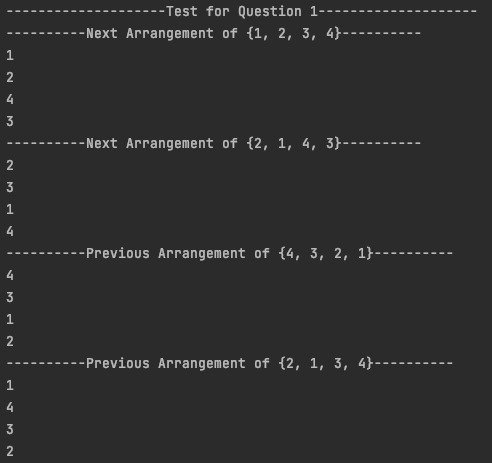
\includegraphics[width=\textwidth]{q1_output}
    \caption{输出结果}
    \label{q1_output}
  \end{figure}

  对于第二问,设计了三个样例,分别是集合$\{1, 2, 3, 4\}, \{5, 7, 9\}, \{7, 9, 5, 1\}$。若要测试其他样例,可以修改源代码中\verb|testForQuestion2|函数并在\verb|main|函数中调用。得到结果如图\ref{q2_output}所示。

  \begin{figure}
    \centering
    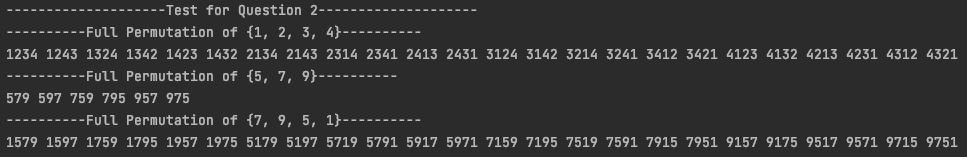
\includegraphics[width=\textwidth]{q2_output}
    \caption{输出结果}
    \label{q2_output}
  \end{figure}

  对于第三问,首先对\verb|nextArrange|函数和\verb|previousArrange|函数测试排列1431,再对序列[1, 1, 3, 4]与[1, 1, 2, 3, 4, 4, 4, 5]分别输出其全排列。两个测试样例的迭代次数(即全排列数)应分别为$\frac{4!}{2!} = 12, \frac{8!}{2!\times 3!} = 3360$。得到结果如图\ref{q3_output}所示。

  \begin{figure}
    \centering
    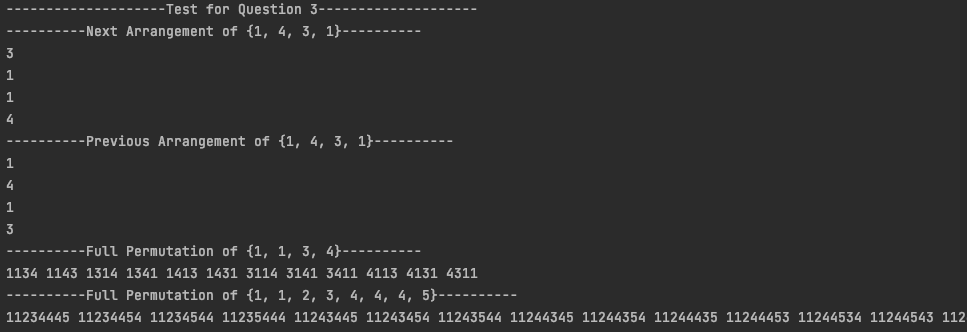
\includegraphics[width=\textwidth]{q3_output}
    \caption{输出结果(部分)}
    \label{q3_output}
  \end{figure}

\section*{主要函数源代码}

\begin{itemize}
  \item \verb|long factorial(int number)|用于计算\verb|number|的阶乘;
  \item \verb|void nextArrange(Integer[] nums)|用于计算排列\verb|nums|的后一个排列(适用于包含重复数字的场景);
  \item \verb|void previousArrange(Integer[] nums)|用于计算排列\verb|nums|的前一个排列(适用于包含重复数字的场景);
  \item \verb|fullPermutation(Set<Integer> set)|用于输出集合\verb|set|的全排列;
  \item \verb|fullPermutationWithRepeatedElem(Integer[] nums, int numbers_of_arrangements)|用于输出序列\verb|nums|的全排列,其中全排列个数为\verb|numbers_of_arrangements|。
\end{itemize}

\lstset{language=java}
  \begin{lstlisting}
    public class Main {
        public static long factorial(int number)
        {
            if (number <= 1)
                return 1;
            else
                return number * factorial(number - 1);
        }

        private static void nextArrange(Integer[] nums)
        {
            for (int i = nums.length - 1; i > 0; i--)
            {
                if (nums[i] > nums[i - 1])
                {
                    Integer temp = nums[i - 1];
                    Integer[] sorted_nums = new Integer[nums.length - i];
                    boolean is_sorted = false;
                    for (int j = i; j < nums.length; j++)
                    {
                        if ((j + 1 == nums.length || nums[j + 1] <= temp) && !is_sorted)
                        {
                            nums[i - 1] = nums[j];
                            nums[j]  = temp;
                            is_sorted = true;
                        }
                        sorted_nums[nums.length - j - 1] = nums[j];
                    }
                    System.arraycopy(sorted_nums, 0, nums, i, sorted_nums.length);
                    break;
                }
            }
        }

        private static void previousArrange(Integer[] nums)
        {
            for (int i = nums.length - 1; i > 0; i--)
            {
                if (nums[i] < nums[i - 1])
                {
                    Integer temp = nums[i - 1];
                    Integer[] sorted_nums = new Integer[nums.length - i];
                    boolean is_sorted = false;
                    for (int j = i; j < nums.length; j++)
                    {
                        if ((j + 1 == nums.length || nums[j + 1] >= temp) && !is_sorted)
                        {
                            nums[i - 1] = nums[j];
                            nums[j]  = temp;
                            is_sorted = true;
                        }
                        sorted_nums[nums.length - j - 1] = nums[j];
                    }
                    System.arraycopy(sorted_nums, 0, nums, i, sorted_nums.length);
                    break;
                }
            }
        }

        private static void fullPermutation(Set<Integer> set)
        {
            Integer[] nums = set.toArray(new Integer[0]);
            Arrays.sort(nums);
            long fact = factorial(nums.length);
            for (long i = 0; i < fact; i++)
            {
                for (Integer num : nums) {
                    System.out.print(num);
                }
                System.out.print(' ');
                nextArrange(nums);
            }
            System.out.println();
        }

        private static void fullPermutationWithRepeatedElem(Integer[] nums, int numbers_of_arrangements)
        {
            Arrays.sort(nums);
            for (long i = 0; i < numbers_of_arrangements; i++)
            {
                for (Integer num : nums) {
                    System.out.print(num);
                }
                System.out.print(' ');
                nextArrange(nums);
            }
            System.out.println();
        }
    }
  \end{lstlisting}

\end{document}